\chapter{Implementation}
\label{cha:Implementation}


\section{Generalising the Codebase}
\label{sec:Generalising the Codebase}
The simulator for this project was created using the AIM simulator codebase \citep{AIMWebsite}, adapted so that new simulations can be run with the GUI without affecting the existing work. This was a project restriction imposed for research purposes. By working with the AIM simulator codebase we can determine whether it will be a good codebase to continue expanding upon for future AV projects. The project: 'A self-organising approach to autonomous vehicle car park management using a message-based protocol' \todo{Add reference}, also uses simulators built using AIM. Each simulator work alongside both the AIM and Merge simulations whilst being completely independent; removing their code would not affect the running of the other simulators. To enable this I worked closely with their project lead to generalise the codebase, breaking out useful shared features so that they can be accessed by all simulator types.



To generalise the codebase we refactored key classes into separate general and AIM specific classes. The general classes can be expanded to create other simulator specific classes, whilst the AIM specific classes maintain the functionality of the original simulator. This helps to reduce code duplication when developing new simulators.

All class diagrams were created using IntelliJ IDEA 15.0.3 internal diagram tool. Figure \ref{fig:classDiagramKey} provides a key for understanding these diagrams.

\begin{figure}[htb]
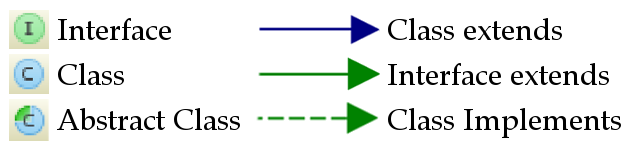
\includegraphics[width=\textwidth]{classDiagrams/classDiagramKey.png}
\caption{Key for the class diagrams in this report.}
\label{fig:classDiagramKey}
\end{figure}

\newtext{Refactoring the AIM codebase was more difficult that originally expected and many changes were made. For brevity, I have only described one of the key parts of the refactor, changing the class structure for classes in \emph{aim4.vehicle}. Appendix \ref{sec:Generalising the Codebase Appendix} provides detailed coverage of both this change, and changes made to some of the other areas of the AIM codebase.}

\todo{Describe this change}.

\section{GUI}
\label{sec:GUI}

\section{Map}
\label{sec:Map}

\section{Simulation}
\label{sec:Simulation}

\section{Merge Schemes}
\label{sec:Merge Schemes}

\section{Results Production}
\label{sec:Results Production}

\section{Testing}
\label{sec:Testing}

\subsection{Unit Testing}
\label{subsec:Unit Testing}
Unit tests were mostly used to ensure getter and setter methods worked as expected. However, some unit tests were used to verify the behaviour of classes. To do this I used Mockito \citep{MockitoWebsite} to mock the behaviour of objects used by the test class so that I could prompt the test class into producing the expected results.

\subsection{Integration Tests}
\label{subsec:Integration Tests}

